\documentclass[12pt, twoside]{article}
\input{../preamble}

\fancyhead[LO]{La Scuola d'Italia / Dr.\ Huson / IB Math \\* 13 May 2026}
\fancyhead[RO]{\fbox{\begin{minipage}{6cm}\footnotesize First \& Last name:\\[0.5cm]\end{minipage}}}
\fancyfoot[C]{\thepage}

\begin{document}
\subsubsection*{7.10 PreQuiz: Logarithmic and Exponential Functions
(calculator)}

\begin{enumerate}[itemsep=0.15cm]

%--- Problem 1: Reading a transformed log graph [6 marks] ---
\item[1.] [Maximum mark: 6]

The graph of $f(x) = \log_{3}(x + 1) + 2$ is shown below.

\begin{center}
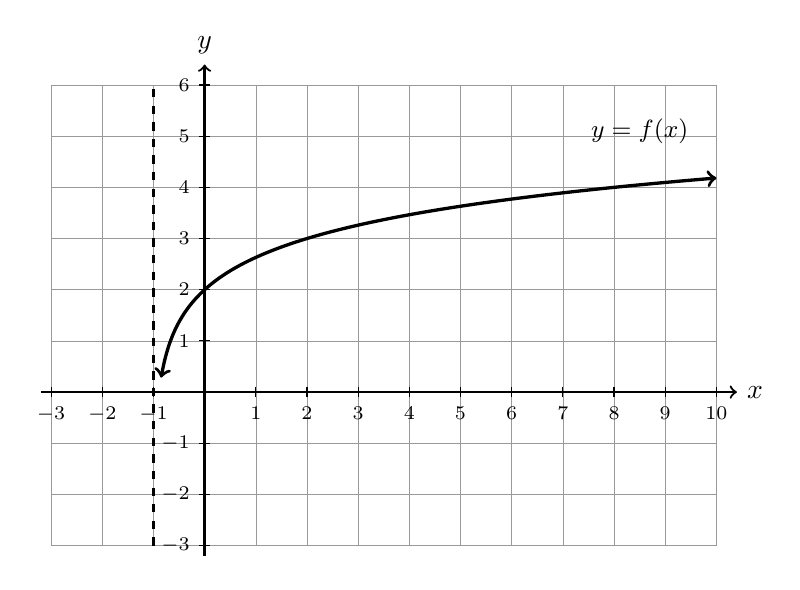
\begin{tikzpicture}[scale=0.65]
  % grid
  \draw[very thin, gray!80] (-3,-3) grid (10,6);
  % axes
  \draw[->, thick] (-3.2,0) -- (10.4,0) node[right] {$x$};
  \draw[->, thick] (0,-3.2) -- (0,6.4) node[above] {$y$};
  % tick labels
  \foreach \x in {-3,-2,-1,1,2,3,4,5,6,7,8,9,10}
    \draw (\x,0.1) -- (\x,-0.1) node[below, font=\scriptsize] {$\x$};
  \foreach \y in {-3,-2,-1,1,2,3,4,5,6}
    \draw (0.1,\y) -- (-0.1,\y) node[left, font=\scriptsize] {$\y$};
  % asymptote dashed
  \draw[dashed, thick] (-1,-3) -- (-1,6);
  % curve
  \draw[<->, very thick, domain=-0.85:10, samples=200, smooth]
    plot (\x, {ln(\x+1)/ln(3) + 2});
  \node[font=\small] at (8.5, 5.1) {$y = f(x)$};
\end{tikzpicture}
\end{center}

\begin{enumerate}[itemsep=0.1cm]
  \item Write down the equation of the vertical asymptote of $f$.
  \hfill [1]
  \item Find the $x$-intercept of the graph of $f$. \hfill [3]
  \item Write down the range of $f$. \hfill [1]
  \item State the coordinates of the point on the graph of $f$ whose
  $x$-coordinate is $8$. \hfill [1]
\end{enumerate}

\begin{tikzpicture}
  \draw (-0.6,0) rectangle (11,7);
  \foreach \y in {1,2,...,6} \draw[dotted] (0,\y)--(10.5,\y);
\end{tikzpicture}

\newpage

%--- Problem 2: Exponential function and its inverse [6 marks] ---
\item[2.] [Maximum mark: 6]

Let $g(x) = 4 \cdot 2^{\,x - 1} - 3$.

\begin{enumerate}[itemsep=0.1cm]
  \item Write down the equation of the horizontal asymptote of
  $y = g(x)$. \hfill [1]
  \item Find $g(3)$. \hfill [2]
  \item Find an expression for $g^{-1}(x)$. \hfill [3]
\end{enumerate}

\begin{tikzpicture}
  \draw (-0.6,0) rectangle (11,13);
  \foreach \y in {1,2,...,12} \draw[dotted] (0,\y)--(10.5,\y);
\end{tikzpicture}

\newpage

%--- Problem 3: Continuous exponential growth [6 marks] ---
\item[3.] [Maximum mark: 6]

The number of registered users of a new social network is modelled by
$$N(t) \;=\; 8000\, e^{\,k t}, \qquad k > 0,$$
where $t$ is the number of years after launch. After $3$ years there
are $24\,000$ registered users.

\begin{enumerate}[itemsep=0.1cm]
  \item Find the value of $k$. Give your answer in the form
  $\dfrac{1}{3}\ln a$, where $a \in \mathbb{Z}^{+}$. \hfill [2]
  \item Find the number of users $7$ years after launch, correct to
  the nearest integer. \hfill [2]
  \item Find the time, in years, at which the number of users first
  reaches $72\,000$. \hfill [2]
\end{enumerate}

\begin{tikzpicture}
  \draw (-0.6,0) rectangle (11,11);
  \foreach \y in {1,2,...,10} \draw[dotted] (0,\y)--(10.5,\y);
\end{tikzpicture}

\newpage

%--- Problem 4: Compound interest [6 marks] ---
\item[4.] [Maximum mark: 6]

Sofia invests \$2500 in an account that pays interest of $4\,\%$ per
annum, compounded annually. No further deposits or withdrawals are
made.

\begin{enumerate}[itemsep=0.1cm]
  \item Show that the value of the account at the end of the first
  year is \$2600. \hfill [1]
  \item Find the value of the account at the end of $10$ years,
  correct to the nearest cent. \hfill [2]
  \item Find the smallest number of full years required for the value
  of the account to first reach \$5000. \hfill [3]
\end{enumerate}

\begin{tikzpicture}
  \draw (-0.6,0) rectangle (11,11);
  \foreach \y in {1,2,...,10} \draw[dotted] (0,\y)--(10.5,\y);
\end{tikzpicture}

\newpage

%--- Problem 5: Logarithmic scale (Richter) [5 marks] ---
\item[5.] [Maximum mark: 5]

The Richter magnitude $M$ of an earthquake is related to its intensity
$I$ by
$$M \;=\; \log_{10}\!\left(\dfrac{I}{I_{0}}\right),$$
where $I_{0}$ is a fixed reference intensity.

\begin{enumerate}[itemsep=0.1cm]
  \item Earthquake $A$ has magnitude $M = 5.4$. Find the value of
  $\dfrac{I}{I_{0}}$ for earthquake $A$. Give your answer in the
  form $a \times 10^{k}$, where $1 \le a < 10$ and $k \in
  \mathbb{Z}$. \hfill [2]
  \item Earthquake $B$ is $500$ times more intense than earthquake
  $A$. Find the magnitude of earthquake $B$, correct to three
  significant figures. \hfill [3]
\end{enumerate}

\begin{tikzpicture}
  \draw (-0.6,0) rectangle (11,12);
  \foreach \y in {1,2,...,11} \draw[dotted] (0,\y)--(10.5,\y);
\end{tikzpicture}

\newpage

%--- Problem 6: Light absorption (exponential decay) [4 marks] ---
\item[6.] [Maximum mark: 4]

The intensity of light at depth $d$ metres below the surface of a
lake is modelled by
$$L(d) \;=\; L_{0}\, e^{-0.32\, d}$$
where $L_{0}$ is the intensity at the surface.

\begin{enumerate}[itemsep=0.1cm]
  \item Find the percentage of the surface intensity that remains at
  a depth of $4$ metres. \hfill [2]
  \item Find the depth, in metres, at which the intensity has fallen
  to half of its surface value. Give your answer correct to three
  significant figures. \hfill [2]
\end{enumerate}

\begin{tikzpicture}
  \draw (-0.6,0) rectangle (11,12);
  \foreach \y in {1,2,...,11} \draw[dotted] (0,\y)--(10.5,\y);
\end{tikzpicture}

\end{enumerate}
\end{document}
